%% Style file for MECH MSc thesis. 
\documentclass[11pt,a4paper]{article}

\usepackage[a4paper, top=25.4mm, bottom=25.4mm, left=19.1mm, right=19.1mm, footskip=8mm]{geometry}
% \usepackage[skip=8pt, indent=20pt]{parskip}
\usepackage[skip=7pt]{parskip}
\usepackage[list=true, listformat=simple]{subcaption}
\usepackage[usestackEOL]{stackengine}
\usepackage{graphicx}
\usepackage{float}
\usepackage{fancyhdr}
\usepackage{gensymb}
\usepackage{amsthm}
\usepackage{amsmath}
\usepackage{amsfonts}
\usepackage{multirow}
\usepackage[hidelinks]{hyperref}
\usepackage{titlesec}
\usepackage{xurl}
\usepackage{indentfirst}
\usepackage{sectsty}
\usepackage{everypage}
\usepackage{times}
\usepackage{cite}
\usepackage{subcaption}
\usepackage{textcomp}

% Change subfigure caption into fontsize 9
\usepackage{caption}
\usepackage{subcaption}
\DeclareCaptionFont{eight}{\fontsize{9}{10}\selectfont}
\captionsetup[subfigure]{font=eight}

% Frame for Cover Page
\usepackage{tikz}
\usetikzlibrary{calc}


% ########### Header and footer ###########
% Defining marks
\renewcommand{\sectionmark}[1]{\gdef\leftmark{#1}}
\renewcommand{\subsectionmark}[1]{\markright{#1}}

\fancypagestyle{coverpage}{
    \fancyhf{}
    \fancyfoot[C]{}
    \renewcommand{\headrulewidth}{0pt}
}

\fancypagestyle{firstpage}{
    \fancyhf{}
    \fancyfoot[C]{\thepage}
    \renewcommand{\headrulewidth}{0pt}
}

\fancypagestyle{fancy}{
    \fancyhf{}
    \fancyhead[L]{UCL Mechanical Engineering}
    \fancyhead[C]{MSc Thesis}
    \fancyhead[R]{AY23-24}
    \fancyfoot[C]{\thepage}
    \renewcommand{\headrulewidth}{0pt}
}

\setlength{\headheight}{13.6pt}
% Use fancy page style unless otherwise specified
\pagestyle{fancy}

% ########### Maths environment spacing ###########

% Redefining space around equation environment
\let\equationOriginal\equation
\let\endequationOriginal\endequation
\renewenvironment{equation}{
    \vspace{-4mm}
    \equationOriginal}
{
\endequationOriginal
\vspace{-7mm}
}

% Redefining space around align environment
\let\alignOriginal\align
\let\endalignOriginal\endalign
\renewenvironment{align}{
    \vspace{-7mm}
    \alignOriginal}
{
\endalignOriginal
\vspace{-8mm}
}

% Redefining space around subequations environment
\let\subequationsOriginal\subequations
\let\endsubequationsOriginal\endsubequations
\renewenvironment{subequations}{
    \subequationsOriginal}
{
\endsubequationsOriginal
\vspace{1mm}
}

% ########### Other ###########

% Biblography spacing
\let\OLDthebibliography\thebibliography
\renewcommand\thebibliography[1]{
  \OLDthebibliography{#1}
  \setlength{\parskip}{0pt}
  \setlength{\itemsep}{5pt plus 0.3ex}
}

% Spacing around headings
\setlength{\parindent}{0pt}
\titlespacing*{\section}{0pt}{5pt}{5pt}
\titlespacing*{\subsection}{0pt}{5pt}{5pt}

% Other spacing
\setlength{\parindent}{2.5mm} % Interparagraph
\setlength{\skip\footins}{8mm} % Footnotes
\setlength{\columnsep}{5mm} % Column separation

% Section formatting
\sectionfont{\centering\MakeUppercase}

% Use roman numerals to count to tables
\renewcommand{\thetable}{\Roman{table}}

% Change the figure and table captions
\captionsetup[table]{labelfont=bf, labelsep=period}
\captionsetup[figure]{labelfont=bf, labelsep=period}

\begin{document}

\thispagestyle{coverpage}

\begin{tikzpicture}[remember picture, overlay]
    \draw[line width = 2.5pt]
    ($(current page.north west) + (13mm,-17mm)$) rectangle ($(current page.south east) + (-13mm,50mm)$);
\end{tikzpicture}

\begin{center}

    \Huge Bayesian Deep Learning Based Semantic Segmentation for Marine Environments

    % \Huge Enhancing USV Visual Detection with \\ Bayesian SegNet\\
    % \vspace{3mm}
    % \huge Deep Learning-Based Semantic Segmentation for \\ Marine Environments under Dataset Scarcity
    
    \vspace{22mm}
    
    \Large A thesis submitted for the degree of Masters of Science in \\
    \Large Power Systems Engineering  \\
    \Large by  \\
    \Large Zehao Ye, BEng (Hons.)
    
    \vspace{20mm}

    \Large Department of Mechanical Engineering  \\
    \Large University College London

    \vspace{20mm}

    \begin{minipage}[t]{0.8\textwidth}
        \centering
        \Large I, Zehao Ye, confirm that the work presented in this thesis is my own. Where information has been 
        derived from other sources, I confirm that this has been specified in the thesis.
    \end{minipage}

    \vspace{20mm}

    \Large \today
    
    {\raggedleft\vfill\itshape\Longstack{
    Student number: 23119333  \\
    Total number of pages: 19
    % For more accurate results use the following
    % https://app.uio.no/ifi/texcount/online.php
    % This won't be checked and there is no limit anyway, so use the built in counter in Overleaf
    }\par}

    \vspace{10mm}
    \begin{minipage}[t]{0.7\textwidth}
        \centering
        \large I give permission to UCL to make this report public after the end of my studies, so UCL students and staff can access it.
    \end{minipage}
    \vspace{2mm}

    % Leave one of these uncommented to show your choice.
    \makebox[0pt][l]{$\square$}\raisebox{0.15ex}{\hspace{0.1em}$\checkmark$} YES \hspace{15mm} \makebox{$\square$} NO

    % \makebox{$\square$} YES \hspace{15mm} \makebox[0pt][l]{$\square$}\raisebox{0.15ex}{\hspace{0.1em}$\checkmark$} NO

\end{center}

\newpage
\setcounter{page}{1}
\thispagestyle{firstpage}

\begin{center}
    \vspace*{-20mm}
    \huge Bayesian Deep Learning Based Semantic Segmentation for Marine Environments\\
    \vspace{5mm}
    \large Zehao Ye  \\
    \large MSc Power Systems Engineering  \\
    \large UCL Mechanical Engineering  \\
    \large London WC1E7JE  \\
    \vspace{3 mm}
    \large \today
\end{center}

\begin{abstract}
    This study explores the application of Bayesian SegNet to enhance semantic segmentation for Unmanned Surface 
    Vehicles (USVs), particularly by providing uncertainty estimation to improve robustness in novel environments. 
    Addressing the challenge posed by limited maritime semantic segmentation datasets, the Bayesian SegNet model 
    demonstrated significant improvements over the non-Bayesian baseline, with a 1.3\% increase in Precision 
    ($\mathbf{Pr}$) and a 6.5\% improvement in F1 score ($\mathbf{F1}$). Furthermore, Bayesian SegNet outperformed 
    traditional SegNet in uncertainty estimation, as shown through entropy-based analysis, and exhibited superior 
    generalization capabilities. This was particularly evident in the evaluation of the OASIs dataset, where Bayesian 
    SegNet achieved a 39.77\% higher $\mathbf{F1}$ compared to SegNet, underscoring its ability to make strong 
    inferences in data-scarce conditions. Beyond maritime applications, the methodologies and outcomes of this 
    study hold potential benefits for other USV-related fields where uncertainty estimation and generalization 
    are critical. However, the study acknowledges the need for further refinement in parameter tuning and broader 
    dataset testing to fully leverage the advantages of Bayesian SegNet. Future research should also explore 
    alternative architectures to optimize computational efficiency, given the resource-intensive nature of Monte 
    Carlo sampling required by Bayesian SegNet.
\end{abstract}

\textbf{Keywords:} Semantic segmentation; Deep learning; Bayes methods; Unmanned Surface Vehicles (USVs); 
Uncertainty; SegNet; Obstacle Detection; Convolutional neural networks; MC-dropout; variational inference.
\section{Introduction}
Unmanned Surface Vehicles (USVs) play a crucial role in commercial shipping\cite{USVshipping}, environmental 
and climate monitoring\cite{USVenvmonitor}, seabed mapping\cite{USVseabedmap}, surveillance and infrastructure 
inspection\cite{USVbridgeinspection}. USVs and AUVS (autonomous underwater vehicles) share similar benefits, 
particularly in reducing the need for personnel to operate in hazardous environments, thereby enhancing safety 
and security and lowering operational costs for maritime tasks. However, AUVs are limited in range and flexibility 
due to their reliance on the mother ship for positioning support\cite{AUV}. In contrast, USVs can operate over 
a wider range with greater precision, offering increased autonomy and adaptability in complex environments 
\cite{USVoverview}. 

As the advantages of USVs become increasingly evident, navigation has emerged as a critical area of 
research. Due to the expansive spatial scale of the marine environment, LiDAR Point Cloud systems commonly 
used in UGVs (unmanned ground vehicles) are not suitable for USVs \cite{lidarpointcloud}. Therefore, cameras 
are employed as sensing modules for USVs due to their lightweight, low-power, and high-information-density 
characteristics \cite{MODS}. Additionally, a perception module is needed to extract useful information from 
high-information-density images through computer vision \cite{perceptionmodule}. Semantic segmentation, which 
provides pixel-level semantic information, is particularly valuable as it helps intelligent systems understand 
spatial positions and make critical decisions \cite{SSsurvey}. This approach, which has been favored in autonomous 
driving\cite{autodrive1}, \cite{autodrive2}, is applicable to USVs with deep learning techniques.

However, using semantic segmentation on USVs presents two main challenges. First, the accuracy of semantic 
segmentation declines when USVs encounter novel scenarios. Most deep learning models for semantic segmentation 
produce point estimates as outputs without providing confidence levels \cite{evaluateBDL}, which can lead to 
errors in novel environments. For example, the autonomous driving system mistakenly identified a plastic bag as a 
rock, resulting in an unnecessary emergency brake \cite{autodrive-mistake}.
% two African Americans were mistakenly identified as gorillas by an image classification system \cite{USAtoday}. 
If models could provide lower confidence for uncertain predictions, 
such issues could be mitigated. Secondly, there is a scarcity of per-pixel semantically labelled marine environment 
databases. Due to the complexity of marine environments, collecting marine datasets is challenging, and the 
available marine datasets are less than those for land environments \cite{CamVid}, \cite{Cityscapes}, 
\cite{landsemanticdataset}. The requirement for per-pixel semantic labelling further increases the cost of marine 
datasets. 

Probabilistic outputs can be derived using the softmax function as the activation function at the output layer, 
or through more complex methods like particle filters to assist in modelling uncertainty in computer vision as a 
measure of confidence \cite{particlefilter}. However, these methods are not based on deep learning and cannot 
achieve state-of-the-art performance \cite{resnet}. Bayesian deep learning approaches have proven effective 
for capturing uncertainty in semantic segmentation, offering a more refined way to model uncertainty 
\cite{whatuncertaintydoweneed}. Additionally, Bayesian deep learning can also address dataset scarcity by 
incorporating epistemic uncertainty to reflect confidence in novel scenarios and using prior distributions 
for regularization, thus preventing overfitting \cite{overfitting}. 

In selecting the deep learning architecture, the VGG16-based SegNet approach was chosen due to the availability 
of existing Bayesian SegNet methodologies that can be leveraged \cite{VGG,SegNet}. The VGG architecture, being 
simpler compared to alternatives like ResNet, is easier to implement and serves well as a foundational model for 
research \cite{vggcompare}. 

The aim of this research is to enhance the visual detection capabilities of USVs by utilizing Bayesian 
SegNet for semantic segmentation in marine environments. This demonstrates that Bayesian SegNet 
can provide robust uncertainty estimates, enhancing reliability in complex and dynamic marine environments. 
Additionally, this approach addresses the challenges posed by dataset scarcity, improving the performance of 
USV perception systems in novel scenarios.

The remainder of this thesis is structured as follows. Section \ref{section:LR} reviews and discusses the most 
relevant prior research in the field. A comprehensive overview of the methodology employed for semantic segmentation
is provided in Section \ref{sectino:Methodology}. Evaluation metrics are presented in Section \ref{section:results}, 
along with a multidimensional performance comparison. Section \ref{section:discussion} analyses the evalaution 
performance and proposes future research directions, while Section \ref{section:conclusion} offers a comprehensive 
conclusion.
\section{Literature Review}
\label{section:LR}
\subsection{Maritime Semantic Segmentation for USV}
USVs are comprised of several critical modules, including the sensing module, perception module, path planning 
module, and control module \cite{MODS}. Within the perception module, the capacity for environmental perception 
is of paramount importance. Given the physical constraints of small USVs, utilizing cameras as the foundational 
sensing component is a more viable solution \cite{lightsensor1}, \cite{lightsensor2}. In camera-based collision 
avoidance systems for USVs, it is essential to detect both static and dynamic obstacles within the environment. 
Traditional object detection algorithms, however, often fall short in accuracy and provide insufficient 
decision-making information for the path planning module \cite{SSsurvey}. In contrast, semantic segmentation is 
capable of effectively bridging the semantic gap between low-level features and high-level semantics, thereby 
enabling more precise environmental perception.

Another significant challenge in environmental perception for USVs is the complexity of the surrounding 
maritime environment. Many maritime object detection algorithms operate under the assumption that obstacles 
are clearly distinguishable from their background \cite{marineobjdetect1}, \cite{marineobjdetect2}. However, this 
assumption often fails in practice due to factors such as fog, water surface reflections, lens obstructions, 
and the presence of reflections of objects on the water, all of which can make obstacles visually similar 
to the water surface. Background subtraction methods are also prone to errors due to the constant motion of 
the sea \cite{backsub}. By contrast, semantic segmentation algorithms offer a more effective approach to 
extracting relevant information in such scenarios. Given its advantages, algorithms in the USV perception 
module are increasingly inclined to use per-pixel labelled outputs from semantic segmentation as input for 
the path planning module \cite{MODS}, \cite{WaSR}, \cite{MaSTr1325}, \cite{MODD2}.

Although semantic segmentation has been established as the primary task, the vast number of available algorithms 
necessitates careful consideration when selecting the most appropriate one. Based on the level of supervision, 
semantic segmentation methods can be categorized into supervised, semi-supervised, and unsupervised approaches 
\cite{SSsurvey}. Supervised methods, in particular, provide more controllable performance and higher accuracy 
with less training difficulty when high-quality datasets are available \cite{semisupervised}. As a result, most 
maritime semantic segmentation approaches rely on supervised methods. Context-based methods like PSP-Net 
\cite{PSPNet} and DeepLab3+ \cite{Deeplab3+}, as well as feature-enhancement-based methods such as FCN 
\cite{FCN} and U-Net \cite{UNet}, are widely employed in the USV domain for semantic segmentation within 
supervised learning approaches. The following discussion will focus on these CNN architectures and their 
applications in USV domain.

\subsection{CNN Architectures}
We have discussed the context-based methods like PSPNet \cite{PSPNet} and DeepLab3+ \cite{Deeplab3+}, 
which utilize ResNet \cite{resnet} as their backbone, and feature-enhancement-based methods like FCN utilize 
VGG16 \cite{VGG} as its backbone and U-Net \cite{UNet} built upon FCN. While USV and UGV semantic segmentation 
tasks are similar, USV technology lags behind UGV technology \cite{MaSTr1325}. Therefore, applying methods from 
the UGV field can be highly beneficial for USVs. In the UGV domain, deconvolution-based methods, with SegNet 
\cite{SegNet} being a notable architecture, are used for semantic segmentation. This section will discuss the 
potential applications of PSPNet, DeepLab3+, U-Net, and SegNet, as well as their potential in the USV domain.

PSPNet, introduced in 2017 by Zhao et al.\cite{PSPNet}, quickly garnered attention in the field of image 
segmentation. Sun et al.\cite{pspnet-ugv} developed an algorithm based on this architecture for image 
segmentation in autonomous driving under rainy conditions. Besides, Zhu et al.\cite{pspnet-cad} applied PSPNet 
to coronary angiography image segmentation, achieving more accurate results than those obtained with U-Net. 
In the USV domain, Yin et al. \cite{pspnet-shoreline} utilized this architecture to develop a shoreline 
recognition algorithm.

U-Net was introduced in 2015 by Ronneberger et al. \cite{UNet} and has since spawned numerous derivative 
architectures \cite{h-dense-unet,3dunet,unet++}. It is particularly widely used in the field of medical 
image segmentation \cite{SSsurvey}. U-Net has been applied to various image modalities, including Magnetic 
Resonance Imaging (MRI), Computed Tomography (CT), Retinal Fundus Imaging, Microscopy, Dermoscopy, Ultrasound, 
and X-Ray \cite{unet-med-reveiw}.

The DeepLab family leverages atrous convolution to expand the receptive field, allowing it to capture 
multiscale contextual information \cite{Deeplab3+}. Yurtkulu et al. \cite{deeplabv3-ugv} developed an 
extended DeepLabv3 framework tailored for the UGV domain. This precise ability to capture fine details 
has also made DeepLab highly favoured in the medical field, as demonstrated by Azad et al. \cite{deeplabv3+-med}, 
who applied DeepLab3+ for skin lesion detection.

SegNet was initially developed for understanding road and indoor scenes, offering efficiency in memory usage and 
computational time \cite{SegNet}. Over time, it has been applied to tasks such as crack detection \cite{segnet-crack} 
and medical image processing \cite{segnet-med}, demonstrating its versatility. All of these architectures show 
potential for application in the USV domain, or have already been utilized in this context. However, their specific 
performance in USV applications remains largely unexplored. Some researchers have begun comparing the effectiveness 
of these architectures for USV tasks, laying the groundwork for selecting the most suitable option among these four 
major architectures.

In the study of the WaSR algorithm, researchers evaluated the performance of PSPNet, SegNet, and DeepLab3+ 
against WaSR using the MODD2 database \cite{MODD2}, assessing marine semantic segmentation across multiple 
dimensions \cite{WaSR}. While the WaSR algorithm demonstrated high accuracy, its reliance on IMU outputs in the 
decoder limits its applicability in this context. Among the three remaining algorithms, SegNet achieved the 
highest precision and F1 score, whereas PSPNet excelled in recall. Overall, SegNet emerged as the most effective 
algorithm for marine semantic segmentation using the MODD2 dataset. Additionally, in the study on the MaSTr1325 
dataset, researchers utilized U-Net and PSPNet to validate the dataset \cite{MaSTr1325}. The comparison revealed 
that PSPNet outperformed U-Net in terms of Precision (Pr) and F1 Scores. According to Table \ref{tab:SS-compare}, 
SegNet appear to be more suitable architecture for semantic segmentation in marine environments.

% table
\begin{table}[ht!]
    \centering
    \caption{Performance of maritime semantic segmentation in terms of Water-Edge Estimation Error $\mu_{edg}$ in Pixels, 
    as well as Precision (Pr), Recall (Re), and F1 Scores in percentages.}
    \label{tab:SS-compare}
    \begin{tabular}{c|c|c|c|c|c}
    \textbf{Architecture}        & \textbf{Dataset}           & \textbf{$\mu_{edg}$} & \textbf{Pr}(\%) & \textbf{Re}(\%) & \textbf{F1}(\%) \\ \hline
    PSPNet\cite{PSPNet}          & MaSTr1325\cite{MaSTr1325}  & 40.0 & 82.1 & 50.8 & 62.8 \\ \hline
    U-Net\cite{UNet}             & MaSTr1325\cite{MaSTr1325}  & 18.8 & 10.2 & 88.6 & 18.3 \\ \hline
    PSPNet\cite{PSPNet}          & MODD2\cite{MODD2}          & 13.5 & 56.8 & 93.2 & 70.6 \\ \hline
    DeepLab3+\cite{Deeplab3+}    & MODD2\cite{MODD2}          & 13.8 & 64.9 & 84.2 & 73.3 \\ \hline
    \textit{SegNet}\cite{SegNet} & MODD2\cite{MODD2}          & 13.2 & 74.3 & 92.5 & 82.4 \\ \hline
    \end{tabular}
\end{table}

\subsection{Bayesian Deep Learning for Semantic Segmentation}
The previously discussed semantic segmentation architectures share a common challenge, as segmentation results 
often carry inherent uncertainty. Most algorithms represent this uncertainty using the softmax function in the 
output layer. However, this output cannot be considered a true measure of confidence, as algorithms tend to be 
overly confident in their predictions \cite{overconfident}. To address the complexities of the maritime 
environment, USVs require a more robust method to quantify uncertainty, and Bayesian deep learning has gained 
attention for its better calibration in this regard \cite{bnn-tutorial}.

Bayesian Deep Learning (BDL) combines deep learning with Bayesian probability theory to train stochastic neural 
networks using a Bayesian approach \cite{bnn-tutorial}. Theoretically, BDL achieves model averaging through 
posterior sampling, bypassing traditional learning. However, the complexity of the sampling space makes direct 
posterior sampling challenging. Since 2014 \cite{bdl-history}, BDL research has rapidly expanded, and this 
challenge has been addressed by two prominent algorithms: Markov chain Monte Carlo (MCMC) method \cite{MCMC}, 
which provides accurate posterior sampling, and variational inference \cite{VI}, which approximates the posterior. 

MCMC excels in small neural networks by sampling numerous instances and storing them \cite{mcmc-bnn}. 
However, for modern large-scale models, performing exact inference requires processing all data in each iteration, 
making the computational cost prohibitively high. The Stochastic Gradient Markov Chain Monte Carlo (SG-MCMC) 
methods \cite{sgmcmc} and the No-U-Turn Sampler (NUTS) \cite{nuts} are proposed to improve the performance of MCMC. 
However, SG-MCMC is implemented using R packages, while NUTS is available through STAN software \cite{stan}. 
Adapting these methods for semantic segmentation poses significant challenges.

In contrast, variational inference has gained considerable popularity due to its scalability, despite not being 
an exact method \cite{bnn-tutorial}. It has been observed to perform strongly with moderately sized architectures 
but struggles with deep residual networks \cite{resnet}. To address this, Gal and Ghahramani \cite{VIdropout} 
connected this technique to variational inference in Bayesian convolutional neural networks, employing Bernoulli 
distributions over the network's weights. Building on this, Alex Kendall et al. \cite{bayesiansegnet} applied the 
approach to perform probabilistic inference in segmentation models, leading to the development of Bayesian SegNet. 
The architecture of Bayesian SegNet, validated using the CamVid dataset \cite{CamVid} and SUN RGB-D dataset 
\cite{sunrgbd}, demonstrated the capability of dropout variational inference for image segmentation and 
uncertainty quantification.

\subsection{Maritime Environment Dataset}
The training of deep learning models heavily relies on high-quality datasets. Therefore, the next section will 
focus on discussing semantic segmentation datasets for marine environments. First, a comprehensive overview and 
comparison of the existing marine environment datasets will be provided. Then, these datasets will be compared 
with those related to UGVs to identify their limitations. Finally, the potential of Bayesian deep learning to 
address these limitations will be explored.

Several datasets are available for marine semantic segmentation tasks, including MaSTr1325 \cite{MaSTr1325}, 
Mari\-ShipSeg-HEU \cite{marishipseg}, Foggy ShipInsseg \cite{foggy}, Tampere Waterseg \cite{tampere}, and Ocean 
AI Segmentation Initiatives (OASIs) \cite{OASIs}. The images and annotations from these datasets are illustrated 
in Fig.\ref{fig:dataset-compare}. MaSTr1325 is the most widely used dataset in marine semantic segmentation, 
offering a diverse range of weather conditions and times of day. It includes three annotation classes: obstacles 
and environment, water, and sky \cite{MaSTr1325}. In contrast, MariShipSeg-HEU and Foggy ShipInsseg focus 
exclusively on ship segmentation, with only two annotation classes each \cite{marishipseg}, \cite{foggy}. Tampere 
Waterseg is specifically designed for water segmentation, with two annotation classes: water and others 
\cite{tampere}. OASIs provides a more comprehensive segmentation approach, featuring four annotation classes: 
others, sea, land, and sea objects \cite{OASIs}. Additionally, OASIs is organized into three subsets, capturing 
conditions during normal environments, adverse weather, and nighttime. Overall, MaSTr1325 and OASIs are particularly 
notable from the perspective of annotation classes. 

\begin{figure}[ht]
    % MaSTr1325
    \centering
    \begin{subfigure}[b]{0.9\textwidth}
        \centering
        \includegraphics[width=\textwidth]{figures/MaSTr1325/official-annotation.jpg}
        \caption{}
        \label{fig:mastr1325}
    \end{subfigure}
    \hfill
    % MariShipSeg-HEU
    \centering
    \begin{minipage}{0.49\textwidth}
    \begin{subfigure}[b]{0.75\textwidth}
        \centering
        \includegraphics[width=\textwidth]{figures/D_MariShipSeg-HEU.jpg}
        \caption{}
        \label{fig:marishipseg}
    \end{subfigure}
    \hfill
    \end{minipage}
     % Foggy
     \hspace{-0.1\textwidth}
    \begin{minipage}{0.49\textwidth}
    \centering
    \begin{subfigure}[b]{1\textwidth}
        \centering
        \includegraphics[width=\textwidth]{figures/D_Foggy.jpg}
        \caption{}
        \label{fig:foggy}
    \end{subfigure}
    \hfill
    % Tampere
    \begin{subfigure}[b]{1\textwidth}
        \centering
        \includegraphics[width=\textwidth]{figures/D_tampere-waterseg.jpg}
        \caption{}
        \label{fig:tampere}
    \end{subfigure}
    \end{minipage}
    \hfill
    % OASIs
    \centering
    \begin{subfigure}[b]{0.9\textwidth}
        \centering
        \includegraphics[width=\textwidth]{figures/OASIs/official-annotation.png}
        \caption{}
        \label{fig:oasis}
    \end{subfigure}
    \caption{The Annotation of different dataset: (a) MaSTr1325 \cite{MaSTr1325}, (b) MariShipSeg-HEU \cite{marishipseg},
    (c) Tampere Waterseg \cite{tampere}, (d) Foggy ShipInsseg \cite{foggy}, (e) OASIs \cite{OASIs}.}
    \label{fig:dataset-compare}
\end{figure}

Compared to datasets in the UGV domain, such as CamVid \cite{CamVid} and CityScapes \cite{Cityscapes} 
(as shown in Table \ref{tab:dataset-compare}), USV datasets are notably smaller in scale and have fewer annotation 
classes. This highlights the limited availability of marine datasets, which results in models trained on these 
datasets being less effective at handling unseen scenarios. USVs, however, are more likely to encounter novel 
environments due to factors such as varying weather conditions and camera instability from wave-induced motion. 
BDL, with its advanced inference capabilities, offers significant potential to address these challenges and enhance 
model robustness in unpredictable marine settings. In BDL methods, Kendall \cite{whatuncertaintydoweneed} employed 
the CamVid dataset to assess the effectiveness of Bayesian SegNet in uncertainty estimation. Additionally, Mukhoti 
and Gal \cite{evaluateBDL} investigated uncertainty evaluation metrics using the Cityscapes dataset. Despite these 
advancements, no models have yet been trained for marine semantic segmentation in USV domain. This paper proposes 
to harness BDL techniques to enhance the robustness of USV environmental perception by improving uncertainty 
estimation.

% table
\begin{table}[ht!]
    \centering
    \caption{Comparison of size and annotation richness between UGV and USV datasets.}
    \label{tab:dataset-compare}
    \begin{tabular}{c|c|c|c}
    \textbf{Dataset} & \textbf{Field} & \textbf{Number of Annotated Image } & \textbf{Number of Classes for Annotation} \\ \hline
    CamVid \cite{CamVid} & UGV & 701  & 32 \\ \hline
    CityScapes \cite{Cityscapes} & UGV & 5000  & 30 \\ \hline
    MaSTr1325 \cite{MaSTr1325} & USV & 1325  & 4 \\ \hline
    OASIs \cite{OASIs} & UGV & 445 & 4 \\ \hline
    \end{tabular}
\end{table}
\section{Methodology}
\label{sectino:Methodology}
This study employs the MaSTr1325 dataset to train a model using Bayesian SegNet, aiming to deliver semantic 
segmentation results for USVs while also quantifying uncertainty. This approach addresses the issue of dataset 
scarcity by enhancing model robustness. Additionally, the model's performance in unfamiliar environments is 
validated using the OASIs dataset. The following sections will detail the dataset preparation, the principles 
underlying Bayesian SegNet, the techniques for uncertainty estimation, and the evaluation metrics.

\subsection{Dataset Preparation}
The study employs two datasets, MaSTr1325 \cite{MaSTr1325} and OASIs \cite{OASIs}. While both datasets provide 
per-pixel annotations, their labelling schemes differ, as detailed in Table \ref{tab:annot-diff}. The annotation 
scheme followed in this research is based on MaSTr1325, which categorizes images into three classes: obstacles 
and environment, water, and sky. Therefore, it is necessary to modify the annotations in the OASIs dataset to 
align with this classification scheme. The "Sea" category in the OASIs dataset is mapped to the "Water" category, 
while the "Land" and "Sea Object" annotations correspond to the "Obstacle and environment" category. However, 
aligning the "Sky" category necessitates some adjustments.

% table
\begin{table}[h!]
    \centering
    \caption{Annotations of MaSTr1325 and OASIs datasets.}
    \label{tab:annot-diff}
    \begin{tabular}{c|c|c|c}
    \textbf{Dataset} & \textbf{Annotation Format} & \textbf{Pixel Value} & \textbf{Pixel Mapping} \\ \hline
    \multirow{4}{*}{MaSTr1325 \cite{MaSTr1325}} & \multirow{4}{*}{Indexed Image (png)} & 0 & Obstacles and environment \\ \cline{3-4}
    & & 1 & Water \\ \cline{3-4}
    & & 2 & Sky \\ \cline{3-4}
    & & 3 & Ignore region \\ \hline
    \multirow{4}{*}{OASIs \cite{OASIs}} & \multirow{4}{*}{Grayscale Image (png)} & 0 & Others \\ \cline{3-4}
    & & 50 & Sea \\ \cline{3-4}
    & & 100 & Land \\ \cline{3-4}
    & & 150 & Sea Object \\ \hline
    \end{tabular}
\end{table}

The OASIs dataset does not include annotations for the "Sky" category, but in most cases, the "Others" category in 
OASIs corresponds to the "Sky" category. However, there are situations where the camera captures the vessel's hull. 
In the OASIs dataset, the hull is classified under the "Others" category, whereas in the MaSTr1325 dataset, even 
a small portion of the USV hull is annotated as "Obstacle and environment". The comparison of annotations related to 
the vessel hull are illustrated in Fig.\ref{fig:vesselhull}. 
\begin{figure}[ht]
    % MaSTr1325
    \centering
    \begin{subfigure}[b]{0.45\textwidth}
        \centering
        \includegraphics[width=\textwidth]{figures/MaSTr1325/vessul-hull.png}
        \caption{}
    \end{subfigure}
    % OASIs
    \centering
    \begin{subfigure}[b]{0.45\textwidth}
        \centering
        \includegraphics[width=\textwidth]{figures/OASIs/vessul-hull.png}
        \caption{}
    \end{subfigure}
    \caption{The Annotation of USV hull on different datasets: (a) MaSTr1325 Dataset with USV hulls, 
    (b) OASIs Dataset with USV and cargo ship hulls.}
    \label{fig:vesselhull}
\end{figure}

Since the annotations cannot be modified, these portions of the data had to be excluded. After excluding 
annotations that include the vessel hull, the "Others" category in the OASIs dataset can be remapped to the "Sky" 
category. Additionally, the images captured from the perspective of cargo ship significantly differ from those taken 
from the USV perspective. Therefore, these two perspectives were separated and used independently for validation. 
After remapping the OASIs dataset annotations to an indexed image format, they can be directly applied for validation.

\subsection{Bayesian SegNet for Semantic Segmentation}
This study utilizes Bayesian SegNet for USV semantic segmentation. Accordingly, this section will explain 
the SegNet Architecture and principles of Dropout Variational Inference, followed by an overview of uncertainty 
estimation. The flow chart of utilizing Bayesian SegNet for semantic segmentation is illustrated in Fig.
\ref{fig:flowchart}
% figure
\begin{figure}[ht]
    \centering
    \includegraphics[width=0.9\textwidth]{figures/flowchart.png}
    \caption{Flow chart on semantic segmentation of Bayesian SegNet.}
    \label{fig:flowchart}
\end{figure}

SegNet consists of an encoder and a decoder network, with a final output layer. The encoder is made up of 13 
convolutional layers, derived from the VGG16 architecture by removing the fully connected layers. The decoder 
network mirrors the encoder, effectively reversing its operations. The final output layer uses the softmax function 
to produce per-pixel point estimates of classes. Due to the removal of fully connected layers, SegNet is 
significantly more efficient than networks like FCN and DeconvNet that include such layers. Additionally, by 
reusing max-pooling indices, SegNet enhances boundary delineation, which is crucial for improving boundary accuracy 
in semantic segmentation tasks \cite{SegNet}.

 Dropout variational inference is utilized in the Bayesian SegNet architecture to provide probabilistic estimates. 
 In the Bayesian paradigm, the posterior distribution is computed based on the prior, likelihood, and evidence in 
 (\ref{eq:bayes-paradigm}). 

\begin{equation}
    P(\mathbf{W}\mid \mathcal{D})=\frac{P(\mathcal{D}\mid \mathbf{W})P(\mathbf{W})}{P(\mathcal{D})}=\frac{P(\mathcal{D},\mathbf{W})}{\int_{\mathbf{W}} P(\mathcal{D},\mathbf{W}^{\prime})d\mathbf{W}^{\prime}}
    \label{eq:bayes-paradigm}
\end{equation}
\vspace{2mm}

$\mathbf{W}$ represents the weights of the network connections, while $\mathcal{D}$ denotes the training dataset, 
which consists of a series of inputs $\mathbf{X}=\{\mathbf{x}_{1},...,\mathbf{x}_{N}\}$ and their corresponding 
labels $\mathbf{Y}=\{\mathbf{y}_{1},...,\mathbf{y}_{N}\}$.

In contrast, VI involves defining a variational distribution $q_{\phi}(\mathbf{W})$ with parameters $\phi$ to 
approximate the posterior distribution. This method seeks to minimize the Kullback-Leibler divergence ($\mathbb{D}_{\text{KL}}$)
\cite{kldivergence} between the variational distribution and the true posterior distribution to achieve a close 
approximation. The optimal value of the parameter $\phi^*$ is given by (\ref{eq:phi-optimal}).\\
\begin{equation}
    \phi^* = \arg \min_{\phi} \mathbb{D}_{\text{KL}}(q_{\phi}(\mathbf{W}) \parallel P(\mathbf{W}\mid \mathcal{D}))
    \label{eq:phi-optimal}
\end{equation}

In BDL, dropout is treated as part of the variational posterior in convolutional layer $i$ with dimension 
$K\text{ x }K$. The weight matrix $\mathbf{W}_i$ is calculated by applying dropout to the variational parameters 
$\mathbf{M}_i$ and vectors of Bernoulli-distributed random variables $z_i$, as shown in (\ref{eq:dropout}). Although 
the dropout probability $p_i$ can be optimized, it is fixed at 0.5 in this study. \\
\vspace{1mm}
\begin{equation}
\begin{aligned}
    &z_{i,j}\sim\mathrm{Bernoulli}(p_i)\mathrm{~for~}j=1,...,K_i,\\
    &\mathbf{W}_i=\mathbf{M}_i\cdot\mathrm{diag}(\mathbf{z}_i),
    \label{eq:dropout}
\end{aligned}
\end{equation}
\vspace{2mm}

For classification tasks, obtaining the per-pixel labelled image and uncertainty requires multiple Monte Carlo 
samples. The segmentation result is derived from the mean of the output layer across $T$ times of Monte Carlo samples, 
as indicated in (\ref{eq:mc-output}). \\
\vspace{1mm}
\begin{equation}
    p(y=c|\mathbf{x},\mathcal{D})\approx\frac{1}{T}\sum_{t=1}^{T}\mathrm{Softmax}(\mathbf{f}^{\widehat{\mathbf{W}}_{t}}(\mathbf{x}))
    \label{eq:mc-output}
\end{equation}
\vspace{2mm}

In this context, $p(y=c|\mathbf{x},\mathcal{D})$ represents the probability of the output $y$ belonging to the 
annotated class $c$ given the input $x$ after training the model. In this study, the annotation classes are defined 
as $c \in C = \{0,1,2,4\}$. Additionally, $\widehat{\mathbf{W}}_{t}$ denotes the convolutional layer weights 
corresponding to the $\text{t}^{\text{th}}$ sample, which have been adjusted according to the dropout variational 
parameters. 

Additionally, Monte Carlo sampling facilitates the calculation of both epistemic and aleatoric uncertainty within 
the model. Epistemic uncertainty refers to the uncertainty in the model parameters and reflects the model's 
understanding of the data distribution. This type of uncertainty, which arise from the marginal posterior distribution 
of the weights, can be mitigated by acquiring more training data. In contrast, aleatoric uncertainty represents the 
inherent noise within the data itself. This type of uncertainty is intrinsic and cannot be reduced by increasing the 
amount of training data. 

It is crucial to estimate both types of uncertainty in semantic segmentation. The estimation formulas for uncertainty 
are illustrated in (\ref{eq:un-est}). Monte Carlo sampling allows for the calculation of the standard deviation 
$\sigma_c$ for each pixel across all classes. By aggregating these deviations, the total standard deviation can be 
obtained to reflect the overall model uncertainty. Aleatoric uncertainty, on the other hand, is assessed by measuring 
the entropy of the distribution. $p_{c}$ represents the probabilistic estimate for class $c$ obtained through Monte 
Carlo sampling. \\
\vspace{-2mm}
\begin{equation}
\begin{aligned}
    \mathbf{EU} = \sum_{c}^{C} \sigma_{c} \ , \quad
    \mathbf{AU} = -\sum_{c}^{C} p_{c} \operatorname{log} p_{c}
    \label{eq:un-est}
\end{aligned}
\end{equation}


\subsection{Evaluation Metrics for Marine Semantic Segmentation}
In semantic segmentation, evaluation metrics plays a crucial role in evaluating model performance. An effective 
metrics facilitates the comparison of different models and enhances the reproducibility of research outcomes. In 
the domain of UGVs, evaluation metrics typically use mean Intersection over Union (mIoU) as the primary evaluation 
metric \cite{CamVid}, \cite{Cityscapes}. However, for marine semantic segmentation, the evaluation protocol must 
address the two distinct challenges faced by USVs: the water edge (shoreline/horizon) detection and the obstacle 
detection \cite{usvbenchmark}. Since the MaSTr1325 dataset lacks shoreline information \cite{MaSTr1325}, this study 
concentrates solely on evaluating the performance of obstacle detection, utilizing metrics of precision 
($\mathbf{Pr}$), recall ($\mathbf{Re}$), and their harmonic mean ($\mathbf{F1}$), as shown in (\ref{eq:metric}).\\
\begin{align}
    \mathbf{Pr} = \frac{TP}{TP+FP} \ , \quad \mathbf{Re} = \frac{TP}{TP+FN} \ , \quad \mathbf{F1} = \frac{2\cdot\mathbf{Pr}\cdot\mathbf{Re}}{\mathbf{Pr}+\mathbf{Re}}
    \label{eq:metric}
\end{align}

True Positive ($TP$) refers to instances where the model correctly identifies a pixel as belonging to the positive 
class. Specifically, for obstacle detection in marine semantic segmentation, a pixel is labeled as a $TP$ when both 
the model's output and the corresponding ground truth annotation are 0. On the other hand, False Positive ($FP$) 
refers to instances where the model incorrectly identifies a pixel as belonging to the positive class. In this 
context, a pixel is labelled as a $FP$ when the model's output is 0, but the corresponding ground truth annotation 
indicates otherwise. Similarly, False Negative ($FN$) refers to instances where the model fails to identify a pixel 
as belonging to the positive class. Here, a pixel is labelled as a $FN$ when the ground truth annotation is 0, but 
the corresponding model's output indicates otherwise.

\section{Results}
\label{section:results}
The objective of this study is to evaluate the effectiveness and robustness of Bayesian SegNet in marine semantic 
segmentation and to assess its predictive capability in novel environments. This evaluation is conducted through 
appropriate metrics. Initially, both Bayesian SegNet and SegNet were trained using the MaSTr1325 training dataset. 
After the models converged, their accuracy was validated against the MaSTr1325 validation dataset based on metrics. 
The performance of these two models was then compared to that of existing semantic segmentation architectures, 
highlighting the Bayesian approach's ability to remove noisy data and improve accuracy. Additionally, this study 
captures both aleatoric and epistemic uncertainty, providing qualitative analysis of these aspects. Finally, the 
Bayesian and non-Bayesian models trained on the MaSTr1325 dataset were used to predict images from the OASIs dataset, 
demonstrating that Bayesian models offer better inference capabilities in novel scenarios. 

\subsection{Model Training and Performance Evaluation}
\label{section:MTPE}
Before training the model, the MaSTr1325 dataset needs to be partitioned for different uses. The dataset was randomly 
split into a 7:2:1 ratio, with 927 images allocated for training, 266 for validation, and 132 for testing, each 
accompanied by corresponding annotations. The size of the training dataset ensures that the model can extract 
sufficient features \cite{MaSTr1325}, while this partitioning strategy helps mitigate the risk of overfitting. 
% figure
\begin{figure}[ht!]
    % subfig1
    \centering
    \begin{subfigure}[b]{\textwidth}
        \centering
        \includegraphics[width=0.32\textwidth]{figures/MaSTr1325/trainloss-nonebayes.jpg}
        \caption{}
        \label{fig:nbs-mastr1325-tl}
    \end{subfigure}
    % subfig2
    \centering
    \begin{subfigure}[b]{0.9\textwidth}
        \centering
        \includegraphics[width=\textwidth]{figures/MaSTr1325/validation-nonebayes.png}
        \caption{}
        \label{fig:nbs-mastr1325-val}
    \end{subfigure}
    \caption{Performance of non-Bayesian SegNet on the MaSTr1325 dataset: 
    (a) Training loss curve using Cross-Entropy Loss, (b) Evaluation metrics curves.}
    \label{fig:nbs-mastr1325-perf}
\end{figure}

During the training of non-Bayesian SegNet using the training dataset from MaSTr1325, the Cross-Entropy Loss for 
each image is computed and accumulated for every iteration within each epoch to form the total training loss. This 
data is used to generate a training loss curve throughout the training process, which is shown in Fig.
\ref{fig:nbs-mastr1325-tl}. However, evaluating model convergence solely based on the training loss curve can be 
misleading, as excessive training may result in overfitting. To address this, the validation dataset is employed 
to help determine whether the model has converged or if overfitting has occurred. Evaluation metrics are used to 
generate an evaluation curve in Fig.\ref{fig:nbs-mastr1325-val}, providing additional insights into the model's 
performance.

For Bayesian SegNet, a distinct method is used for calculating training loss. Specifically, the negative 
log-likelihood loss (NLLL) is computed and averaged, while an accuracy curve for the predictions is also generated, 
as illustrated in Fig.\ref{fig:bs-mastr1325-tl}. Additionally, the validation dataset is used to evaluate the 
model's performance through appropriate evaluation metrics. The resulting metrics curves are depicted in Fig.
\ref{fig:bs-mastr1325-val}.
% figure
\begin{figure}[ht!]
    % subfig1
    \centering
    \begin{subfigure}[b]{\textwidth}
        \centering
        \includegraphics[width=0.75\textwidth]{figures/MaSTr1325/trainloss-bayes.png}
        \caption{}
        \label{fig:bs-mastr1325-tl}
    \end{subfigure}
    % subfig2
    \centering
    \begin{subfigure}[b]{\textwidth}
        \centering
        \includegraphics[height = 5cm, width=0.9\textwidth]{figures/MaSTr1325/validation-bayes.png}
        \caption{}
        \label{fig:bs-mastr1325-val}
    \end{subfigure}
    \caption{Performance of Bayesian SegNet on the MaSTr1325 dataset: 
    (a) Accuracy and training loss curves using NLLL, (b) Evaluation metrics curves.}
    \label{fig:bs-mastr1325-perf}
\end{figure}

In the calculation of evaluation metrics, a threshold of 0.2 is predominantly employed. This implies that if the 
softmax values for all classes are below 0.2, the pixel is labelled as "Unknown." This relatively low threshold 
encourages the algorithm to annotate regions with high uncertainty. However, the optimal threshold should be 
determined through empirical testing. Fig.\ref{fig:eval-threshold} presents the Precision ($\mathbf{Pr}$), 
Recall ($\mathbf{Re}$), and F1 score ($\mathbf{F1}$) for Bayesian and non-Bayesian SegNet models on the MaSTr1325 
validation dataset across varying thresholds.
% figure
\begin{figure}[ht!]
    \centering
    \includegraphics[width=0.9\textwidth]{figures/MaSTr1325/evaluation-threshold.png}
    \caption{,$\mathbf{Pr}$, $\mathbf{Re}$, and $\mathbf{F1}$ comparison for Bayesian and non-Bayesian SegNet models.}
    \label{fig:eval-threshold}
\end{figure}

The performance of the Bayesian SegNet can be compared with other networks trained on the MaSTr1325 dataset. In 
this context, it is compared with the Unet and PSPNet trained by Bovcon et al. \cite{MaSTr1325}, and the SegNet 
model trained in this study. The comparison is illustrated in Table \ref{tab:BS-vs-others}. It can be observed 
that accuracy has improved by 1.3\% compared to the non-Bayesian baseline, achieved by mitigating the impact of 
noisy data. Additionally, a significant reduction in False Negative rates (FNr) has led to a substantial increase 
in Recall. Compared to the other two architectures, the SegNet architecture has demonstrated its superiority in the 
field of maritime semantic segmentation, particularly through its outstanding $\mathbf{F1}$. Overall, the Bayesian 
SegNet architecture not only delivers highly accurate segmentation, but also effectively mitigates the impact of noise 
in the data on accuracy.
% table
\begin{table}[ht!]
    \centering
    \caption{Performance of Bayesian SegNet compared with other models.}
    \label{tab:BS-vs-others}
    \begin{tabular}{c|c|c|c}
    \textbf{Architecture}        & \textbf{Pr}(\%) & \textbf{Re}(\%) & \textbf{F1}(\%) \\ \hline
    Bayesian SegNet              & 81.2 & 97.8 & 87.8 \\ \hline 
    SegNet                       & 79.9 & 87.5 & 81.3 \\ \hline 
    PSPNet\cite{PSPNet}          & 82.1 & 50.8 & 62.8 \\ \hline
    U-Net\cite{UNet}             & 10.2 & 88.6 & 18.3 \\ \hline
    \end{tabular}
\end{table}

\subsection{Uncertainty Estimation}
\label{section:UE}
Fig.\ref{fig:bs-mastr1325-disp} shows segmentation and model uncertainty estmation from Bayesian SegNet on 
MaSTr1325 testing dataset. High epistemic uncertainty is often observed in instances where SegNet generates an 
incorrect class label. 
% figure
\begin{figure}[ht!]
    \centering
    \includegraphics[width=0.9\textwidth]{figures/MaSTr1325/BayesianSegNet-panel.png}
    \caption{Bayesian SegNet on MaSTr1325 testing dataset.}
    \label{fig:bs-mastr1325-disp}
\end{figure} 

In Fig.\ref{fig:error1}, the uncertainty estimation results highlight two areas of notably high 
uncertainty, in addition to the object edges. These areas, marked with red boxes, are associated with distortions 
caused by reflections on the water surface. The area located at the bottom of the image exhibits distortion due 
to sunlight reflecting off the water. However, the point estimate of the model remains unaffected by this distortion 
and correctly assigns the class label. In contrast, the area on the right side of the image, presents some 
misclassifications, which are accompanied by a correspondingly high uncertainty estimation. In Fig.\ref{fig:error2}, 
a different misclassification scenario is observed, where the algorithm incorrectly identifies the wall as water. 
This misclassification may be due to the similar texture or colour patterns between the wall and the water surface, 
or due to poor lighting conditions that obscure the distinguishing features. However, these misclassified areas are 
accompanied by high levels of aleatoric and epistemic uncertainty. Overall, this approach provides a means of applying 
corrective measures in cases of misclassification, thereby enhancing the robustness of the USV perception module. 
% figure
\begin{figure}[ht!]
    % subfig1
    \centering
    \begin{subfigure}[h]{\textwidth}
        \centering
        \includegraphics[width=0.9\textwidth]{figures/MaSTr1325/errorness1.png}
        \caption{}
        \label{fig:error1}
    \end{subfigure}
    % subfig2
    \centering
    \begin{subfigure}[h]{\textwidth}
        \centering
        \includegraphics[width=0.9\textwidth]{figures/MaSTr1325/errorness2.png}
        \caption{}
        \label{fig:error2}
    \end{subfigure}
    \caption{Misclassifications with high uncertainty in different scenarios: 
    (a) Caused by water surface reflection, (b) Caused by wall texture similarity.}
    \label{fig:high-uncertainty}
\end{figure}

Additionally, to assess the potential of uncertainty in enhancing the performance of the perception module, the 
epistemic uncertainty threshold was set. Pixels with epistemic uncertainty exceeding this threshold were 
reclassified into class 4. This method was employed to determine whether integrating uncertainty can effectively 
improve the accuracy of semantic segmentation. In practical USV applications, the information regarding aleatoric 
and epistemic uncertainty should be handled by the path planning module, rather than simply excluding the 
segmentation results for regions with high uncertainty. 

As shown in Table \ref{tab:uncertainty-threshold}, it can be observed that as the threshold decreases, $\mathbf{Pr}$ 
and $\mathbf{F1}$ correspondingly increase, while $\mathbf{Re}$ decreases. Calculating the average number of True 
Positives ($\mathbf{TP_r}$), False Positives ($\mathbf{FP_r}$), and False Negatives ($\mathbf{FN_r}$)  reveals that 
as the threshold decreases, $\mathbf{FN_r}$ gradually increase, while $\mathbf{TP_r}$ and $\mathbf{FP_r}$ decreases. 
The table does not include thresholds of 0.6, 0.7, 0.8, and 0.9 because, in these cases, the maximum epistemic 
uncertainty is less than 0.5. Therefore, the values for thresholds between 0.5 and 1.0 are effectively the same.
% table
\begin{table}[ht!]
    \centering
    \caption{Performance of Bayesian SegNet compared with other models.}
    \label{tab:uncertainty-threshold}
    \begin{tabular}{c|c|c|c|c|c|c}
    \textbf{Epistemic Uncertainty Threshold} & $\mathbf{TP_r}$ &$\mathbf{FP_r}$ & $\mathbf{FN_r}$ & \textbf{Pr}(\%) & \textbf{Re}(\%) & \textbf{F1}(\%) \\ \hline
    1.00 & 14968.86 & 3301.41 & 457.17 & 76.78 & 98.78 & 85.06 \\ \hline 
    0.50 & 14968.86 & 3301.41 & 457.17 & 76.78 & 98.78 & 85.06 \\ \hline 
    0.40 & 14854.52 & 3045.23 & 571.51 & 78.05 & 98.36 & 85.98 \\ \hline
    0.30 & 14630.89 & 2462.62 & 795.14 & 81.08 & 97.50 & 87.69 \\ \hline
    0.20 & 14405.76 & 2009.39 & 1020.27 & 83.59 & 96.50 & 88.80 \\ \hline
    0.10 & 14085.67 & 1580.83 & 1340.36 & 86.21 & 94.85 & 89.56 \\ \hline 
    0.05 & 13858.67 & 1338.45 & 1567.36 & 87.72 & 93.52 & 89.74 \\ \hline 
    \end{tabular}
\end{table}

\subsection{Domain Transfer Evaluation}
\label{section:DTE}
To assess the generalization capabilities, Bayesian SegNet and non-Bayesian SegNet models trained on the 
MaSTr1325 dataset were evaluated using the OASIs dataset \cite{OASIs}. While many studies validate models trained 
on MaSTr1325 using the MODD2 dataset \cite{MODS,MODD2,WaSR}, this approach may have inherent limitations. Both 
datasets 
were collected with USVs in the Gulf of Koper, Slovenia \cite{MaSTr1325}, which might introduce subtle, shared 
features. Consequently, models trained on these datasets may inadvertently learn and rely on these latent 
characteristics, inaccurately representing them as features of the marine environment. To mitigate this issue, 
it is preferable to use marine environment datasets collected from different geographical regions for evaluation. 
Unlike the SMD dataset used by Borja Bovcon and Matej Kristan \cite{WaSR}, the OASIs dataset was chosen for its 
classification of data based on varied collection conditions, which supports a more comprehensive analysis. 

Fig.\ref{fig:bs-oasis-usv} shows segmentation and model uncertainty estimation from Bayesian SegNet 
on OASIs dataset. Each row of images corresponds to a different scenario. The first row (type 1) represents the 
Day-Time Environment, the second row (type 2) represents the Adverse Weather Environment, and the third row (type 3) 
indicates the Night-Time Environment. These categories are defined by the OASIs dataset.
% figure
\begin{figure}[ht!]
    \centering
    \includegraphics[width=0.9\textwidth]{figures/OASIs/BayesianSegNet-usv-panel.png}
    \caption{Bayesian SegNet performance evaluation on USV perspective.}
    \label{fig:bs-oasis-usv}
\end{figure} 

The performance evaluation on the MaSTr1325 validation dataset was conducted using the corresponding evaluation 
metrics. In the domain transfer evaluation, the same metrics were applied to assess the model's performance on the 
OASIs dataset. To facilitate a more detailed comparison, this study further subdivides the OASIs dataset. Since 
the OASIs dataset was captured from two perspectives, it is divided into the perspectives of USV and cargo ship. 
This study evaluates the model's performance across the three types in the OASIs dataset and their corresponding 
perspectives using the defined metrics. The results are compared with SegNet model trained on the MaSTr1325 dataset 
and evaluated on the SMD dataset \cite{WaSR}, which is illustrated in Table \ref{tab:DTEP}. 
% table
\begin{table}[ht!]
    \centering
    \caption{Evaluation on domain transfer performance.}
    \label{tab:DTEP}
    \begin{tabular}{c|c|c|c|c|c|c}
    \textbf{Architecture} & \textbf{Evaluation Dataset} & \textbf{Type} & \textbf{Perspective} & \textbf{Pr}(\%) & \textbf{Re}(\%) & \textbf{F1}(\%) \\ \hline
    \multirow{9}{*}{Bayesian SegNet} & \multirow{9}{*}{OASIs} & \multirow{3}{*}{1} & USV & 68.73 & 84.31 & 72.67 \\  \cline{4-7}
     & &                    & Cargo Ship & 36.55 & 76.45 & 46.79 \\ \cline{4-7}
     & &                    & \textbf{Total} & 60.77 & 82.37 & 66.27 \\ \cline{3-7}
     & & \multirow{3}{*}{2} & USV & 47.27 & 95.74 & 64.36 \\ \cline{4-7}
     & &                    & Cargo Ship & 53.18 & 50.24 & 49.06 \\ \cline{4-7}
     & &                    & \textbf{Total} & 52.57 & 54.95 & 50.60 \\ \cline{3-7}
     & & \multirow{3}{*}{3} & USV & 65.20 & 88.89 & 73.52 \\ \cline{4-7}
     & &                    & Cargo Ship & 30.04 & 70.82 & 37.48 \\ \cline{4-7}
     & &                    & \textbf{Total} & 39.16 & 75.51 & 46.83 \\ \hline
     \multirow{9}{*}{SegNet} & \multirow{9}{*}{OASIs} & \multirow{3}{*}{1} & USV & 28.27 & 65.89 & 33.93 \\  \cline{4-7}
     & &                    & Cargo Ship & 10.93 & 89.98 & 18.78 \\ \cline{4-7}
     & &                    & \textbf{Total} & 24.02 & 71.79 & 30.22 \\ \cline{3-7}
     & & \multirow{3}{*}{2} & USV & 1.69 & 97.17 & 3.32 \\ \cline{4-7}
     & &                    & Cargo Ship & 16.45 & 77.84 & 25.26 \\ \cline{4-7}
     & &                    & \textbf{Total} & 14.92 & 79.84 & 22.99 \\ \cline{3-7}
     & & \multirow{3}{*}{3} & USV & 10.09 & 98.97 & 17.82 \\ \cline{4-7}
     & &                    & Cargo Ship & 8.91 & 96.42 & 15.41 \\ \cline{4-7}
     & &                    & \textbf{Total} & 9.22 & 97.08 & 16.03 \\ \hline
    SegNet & SMD & -- & -- & 31.2 & 76.3 & 44.3 \\ \hline
    \end{tabular}
\end{table}

According to Table \ref{tab:DTEP}, the evaluation using the OASIs dataset shows that the Bayesian SegNet exhibits 
significantly better generalization capabilities compared to SegNet. In all three environments (type 1, 2, and 3), 
Bayesian SegNet achieves higher accuracy than SegNet. Since the SMD dataset does not include images of adverse 
weather (obscured by droplets) or nighttime conditions, the comparison is limited to type 1 evaluation results. 
It is observed that the performance on the OASIs dataset from the perspective of USV is slightly lower than that on 
the SMD dataset, indicating that the OASIs dataset has less similarity to the MaSTr1325 dataset compared to the SMD 
dataset. This lower similarity helps in better evaluating generalization capabilities. The differing performances 
across the three environments will be analysed in detail in Section \ref{section:ADT}.
\section{Discussion}
\label{section:discussion}
In the Discussion, the experimental results are interpreted and analysed. The discussion is organized into three 
main subsections similar with Section \ref{section:results}, which are analysis of model performance, uncertainty 
estimation, and domain transfer. Subsection \ref{section:AMP} focuses on evaluating the model performance in 
comparison with other models. Subsection \ref{section:AUE} examines how uncertainty estimation may enhance the 
robustness of the model for USVs. Subsection \ref{section:ADT} analyses the generalization capabilities of 
Bayesian SegNet Method.

\subsection{Analysis of Model Performance}
\label{section:AMP}
Firstly, the training and evaluation curves presented in Fig.\ref{fig:nbs-mastr1325-perf} do not conclusively 
demonstrate that the SegNet model has converged, nor do they definitively indicate that further training would 
result in overfitting. Theoretically, continued training could be viable. However, the decision to cease further 
training of the SegNet model was predicated on the excessive computational resources consumed by the process. 
According to the log files, training for 200 epochs with a batch size of 4 on an NVIDIA 4090D GPU consumed 
approximately 9.982 hrs, with an average time of 179.67 seconds per epoch. Further training would likely yield 
only marginal improvements whilst requiring significantly more computational resources, rendering it suboptimal 
from a cost-benefit perspective. 

In contrast, the Bayesian SegNet architecture, owing to its use of MC dropout which mitigates overfitting, can 
theoretically be trained indefinitely. In practice, training for 1000 epochs with a batch size of 1 required 12.6 
hours, with an average of 45.36 seconds per epoch. This reduction in computational time is attributable to the 
dropout process severing certain connections, thereby economising on calculations. As evident from Fig.
\ref{fig:bs-mastr1325-perf}, the model appears to have converged around epoch 300, with the subsequent 700 epochs 
yielding relatively limited improvements.

The more severe instability observed in the evaluation curves of the non-Bayesian SegNet model may be mainly 
attributed to the relatively large learning rate during training, which leads to fluctuations in the performance 
metrics during evaluation. In contrast, the Bayesian SegNet model makes the evaluation curve smoother through the 
implementation of smaller learning rate and MC dropout.

Additionally, this study evaluates the performances of models using different softmax thresholds based on the 
evaluation metrics in Fig.\ref{fig:eval-threshold}. The results indicate that while SegNet demonstrates higher 
precision than Bayesian SegNet when the threshold is low, Bayesian SegNet generally outperforms SegNet in other 
scenarios. The lower precision of Bayesian SegNet at lower thresholds may be attributed to the prior distribution, 
which potentially increases the probabilistic weighting of obstacles. This adjustment likely encourages Bayesian 
SegNet to classify more objects as obstacles, resulting in a higher $\mathbf{FP_r}$. 

The evaluation of the model performance has certain limitations. Firstly, it would be advantageous to experiment 
with varying batch sizes during the training of the Bayesian SegNet model to identify the optimal configuration. 
Secondly, exploring modifications to the prior distribution within the Bayesian SegNet algorithm could be valuable 
in determining whether it can enhance precision at lower softmax thresholds. Despite these considerations, the 
Bayesian SegNet model overall demonstrates superior performance when compared to SegNet and other models, making 
it particularly well-suited for maritime semantic segmentation.

\subsection{Analysis of Uncertainty Estimation}
\label{section:AUE}
Compared to the approximate confidence generated by softmax function, Bayesian SegNet offers a more accurate 
uncertainty estimation. Since the softmax probabilistic cannot be directly compared with uncertainty measurands, 
they are converted into entropy and then compared with aleatoric uncertainty, which is also in the form of entropy. 
Subtracting aleatoric uncertainty from the softmax entropy reveals that entropy at the obstacle edges during semantic 
segmentation is notably higher with the softmax function. Owing to resolution limitations, boundaries are difficult 
to delineate, resulting in high uncertainty in these regions. However, aleatoric uncertainty provides a smoother 
transition by better quantifying this uncertainty. As illustrated in Fig.\ref{fig:entropy}, the pixel with the 
highest entropy has a softmax entropy of 0.92025, while the entropy calculated from aleatoric uncertainty is only 
0.4581. The red dots in the image highlight points where there is a significant difference between the two entropy 
values.
% figure
\begin{figure}[ht!]
    \centering
        \centering
        \includegraphics[width=0.9\textwidth]{figures/MaSTr1325/entropy.png}
    \caption{Entropy subtraction for uncertainty estimation comparison.}
    \label{fig:entropy}
\end{figure}

Moreover, there are certain issues associated with uncertainty estimation. Firstly, there is significant overlap 
between epistemic uncertainty and heteroscedastic aleatoric uncertainty, as illustrated in Fig.
\ref{fig:bs-mastr1325-disp}. The underlying reasons for this overlap can be analysed from the perspective of the 
USV image itself and the ground truth labels used in training. 

From the perspective of USV images, at the edges of semantic segmentation, the model struggles to assign a 
definitive label to a pixel due to resolution limitations. This results in high epistemic uncertainty. 
Additionally, these edge regions are more susceptible to factors like lighting, which increases the inherent 
noise during observation, leading to higher heteroscedastic aleatoric uncertainty.

From the perspective of dataset labelling, edge regions in the images are labelled as class 4, which is the unknown 
categories. In the model's prior, class 4 is assigned a value of 0, meaning the model has limited understanding of 
these regions, which results in higher epistemic uncertainty. Correspondingly, due to heteroscedastic aleatoric 
uncertainty capturing inherent noise from the data, these unlabelled regions inherently possess a high degree of 
uncertainty, thus leading to greater heteroscedastic aleatoric uncertainty.

Moreover, leveraging uncertainty to assist USVs in visual enhancement and further improve their robustness remains 
a challenge. As shown in Table \ref{tab:uncertainty-threshold}, setting a threshold for epistemic uncertainty can 
enhance segmentation performance. However, the selection of this specific threshold lacks mathematical justification 
and cannot be quantitatively determined.

\subsection{Analysis of Domain Transfer}
\label{section:ADT}
Bayesian SegNet demonstrated outstanding performance in generalization capabilities evaluation. In the results, 
the OASIs dataset was divided into six subcategories. This section will analyse the performance of Bayesian and 
non-Bayesian models across these six subcategories and compare their generalization performance with the SegNet 
model, which was also trained on the MaSTr1325 dataset and evaluated on the SMD dataset.

In the multi-class scatter plot (Fig.\ref{fig:domain-transfer-disp}), the segmentation performance of various 
architectures across different subcategories is presented. The Bayesian SegNet architecture demonstrates strong 
performance for the USV perspective on the OASIs dataset, achieving an average $\mathbf{F1}$ of 70.21\% across the 
three types, which indicates a balance between precision and recall in semantic segmentation. The semantic segmentations 
of three types are illustrated in Fig.\ref{fig:bs-oasis-usv}. Conversely, when applied to semantic segmentation 
of cargo ship images in the OASIs dataset, the $\mathbf{F1}$ of the Bayesian SegNet architecture shows a decline by 
approximately 30\%. This reduction can be attributed to the lack of similar scenario in the MaSTr1325 dataset. 
The semantic segmentation results for cargo ship perspectives, as shown in Fig.\ref{fig:bs-oasis-cargo}, 
highlight the difficulty of performing inference with BDL on completely novel perspectives, resulting in 
suboptimal performance. However, in these scenarios, the algorithm yields high uncertainty estimates, which 
contribute to the robustness of the USV when navigating entirely novel environments. 
% figure
\begin{figure}[ht!]
    \centering
        \centering
        \includegraphics[width=0.5\textwidth]{figures/OASIs/domain-tranfer-PrRe.png}
    \caption{Domain transfer of different architecture and subcategories.}
    \label{fig:domain-transfer-disp}
\end{figure}
% figure
\begin{figure}[t!]
    \centering
        \centering
        \includegraphics[width=0.9\textwidth]{figures/OASIs/BayesianSegNet-cargo-panel.png}
    \caption{Bayesian SegNet performance evaluation on cargo ship perspective.}
    \label{fig:bs-oasis-cargo}
\end{figure}

Although this study primarily focuses on USVs, the cargo ship perspective was included as a reference due to the 
limited number of USV perspective images available in the OASIs dataset for types 2 and 3. This inclusion serves 
as a reference point and facilitates further investigation into the model's inference capabilities in novel scenarios. 
% figure
\begin{figure}[ht!]
    \centering
    % subfig1
    \begin{subfigure}[h]{0.49\textwidth} \centering
        \includegraphics[width=0.99\textwidth]{figures/OASIs/SegNet-type1-91.png}
        \caption{}
    \end{subfigure} \hspace{-10mm}
    % subfig2
    \begin{subfigure}[h]{0.49\textwidth} \centering
        \includegraphics[width=0.99\textwidth]{figures/OASIs/SegNet-type1-23.png}
        \caption{}
    \end{subfigure}
    % subfig3
    \begin{subfigure}[h]{0.49\textwidth} \centering
        \includegraphics[width=0.99\textwidth]{figures/OASIs/SegNet-type2-29.png}
        \caption{}
    \end{subfigure} \hspace{-10mm}
    % subfig4
    \begin{subfigure}[h]{0.49\textwidth} \centering
        \includegraphics[width=0.99\textwidth]{figures/OASIs/SegNet-type2-24.png}
        \caption{}
    \end{subfigure}
    % subfig5
    \begin{subfigure}[h]{0.49\textwidth} \centering
        \includegraphics[width=0.99\textwidth]{figures/OASIs/SegNet-type3-53.png}
        \caption{}
    \end{subfigure} \hspace{-10mm}
    % subfig6
    \begin{subfigure}[h]{0.49\textwidth} \centering
        \includegraphics[width=0.99\textwidth]{figures/OASIs/SegNet-type3-18.png}
        \caption{}
    \end{subfigure}
    \caption{Semantic Segmentations of SegNet architecture on OASIs dataset: (a)type 1 with USV perspective, 
    (b)type 1 with cargo ship perspective, (c)type 2 with USV perspective, (d)type 2 with cargo ship perspective, 
    (e)type 3 with USV perspective, (f)type 3 with cargo ship perspective.}
    \label{fig:segnet-oasis}
\end{figure}

Regarding the SegNet architecture, the data from Table \ref{tab:DTEP} indicates that $\mathbf{Pr}$,  $\mathbf{Re}$, 
and  $\mathbf{F1}$ of subcategory type 1 from the USV perspectives are comparable to domain transfer analysis with 
SMD as a benchmark. However, for type 2 and 3, there is a notable decrease in $\mathbf{Pr}$ and a concurrent increase 
in $\mathbf{Re}$. This issue arises because SegNet labels a substantial number of pixels as class 0. While this 
results in high $\mathbf{TP_r}$ and low $\mathbf{FN_r}$, it also leads to a significant increase in $\mathbf{FP_r}$. 
In the cargo ship perspective, a similar issue of excessive labelling as class 0 is observed, as detailed in Fig.
\ref{fig:segnet-oasis}. Overall, the performance of SegNet on this dataset falls short of satisfactory segmentation.

Additionally, discrepancies due to different labelling standards also introduce errors. For example, as shown in 
Fig.\ref{fig:seagull}, in the MaSTR1325 dataset, seagulls are categorized as class 0, which is obstacles. However, 
according to the labelling standards of the OASIs dataset, they are not marked as sea objects in the ground truth. 
This discrepancy may also contribute to some degree of error. 
% figure
\begin{figure}[ht!]
    \centering
    % subfig1
    \begin{subfigure}[h]{0.45\textwidth} \centering
        \includegraphics[width=0.99\textwidth]{figures/OASIs/BayesianSegNet-seagull.png}
        \caption{}
    \end{subfigure} \hspace{-1mm}
    % subfig2
    \begin{subfigure}[h]{0.45\textwidth} \centering
        \includegraphics[width=0.99\textwidth]{figures/OASIs/SegNet-seagull.png}
        \caption{}
    \end{subfigure}
    \caption{Different labelling standards between MaSTr1325 and OASIs datasets: 
    (a) Seagulls Identified as Obstacles by Bayesian SegNet, (b) Seagulls Identified as Obstacles by SegNet.}
    \label{fig:seagull}
\end{figure}

Ultimately, further experiments are needed to fully assess the generalization capabilities of Bayesian SegNet. It 
would be beneficial to test the model using other datasets, such as SMD, and to apply various thresholds to filter 
the semantic segmentation results. Additionally, testing Bayesian and non-Bayesian models using the MODD2 dataset 
and associated tools could provide insights into their performance in water segmentation and Water-Edge Estimation 
Error in Pixels ($\mu_{edge}$). The current series of validations demonstrate the unique advantages of the model in 
enhancing the visual processing capabilities and robustness of USVs. However, they do not fully establish that the 
model can replace existing USV technologies or surpass other technologies in all respects.


\section{Conclusion}
\label{section:conclusion}
This study aimed to enhance semantic segmentation for USVs by utilizing Bayesian SegNet to provide uncertainty 
estimation and improve robustness in novel environments, thereby addressing the challenge of limited maritime 
environment semantic segmentation datasets. The results indicate that Bayesian SegNet, by reducing noise in input 
data, improves Precision ($\mathbf{Pr}$) by 1.3\% and increases the F1 score ($\mathbf{F1}$) by 6.5\% compared to the 
non-Bayesian baseline. Additionally, Bayesian SegNet significantly outperforms SegNet in uncertainty estimation, as 
demonstrated through entropy-based analysis. 

Moreover, the Bayesian model shows superior generalization capabilities, with a notable advantage in evaluating 
the OASIs dataset from the USV perspective. The F1 score achieved by Bayesian SegNet surpasses that of SegNet by 
39.77\%, highlighting the strong inference abilities of Bayesian Approach in conditions with limited training data. 
These evaluations further demonstrate that Bayesian SegNet can effectively enhance USV environmental perception 
based on existing trained models in new environments. 

The characteristics of Bayesian SegNet provide USVs with more precise and reliable environmental perception, 
enhancing their autonomous navigation and risk avoidance capabilities in maritime environment. Given the 
ever-changing maritime environment, the coverage of available datasets is inherently limited. By leveraging the 
inference capabilities of the Bayesian approach, this model can effectively perceive a wider range of scenarios 
using limited datasets. As part of the perception module, this model is crucial for the autonomous navigation 
systems of USVs.

Beyond maritime applications, the methods, and findings of this study have the potential to impact other USV-related 
fields where strong environmental perception is essential. For instance, automated navigation in inland waterways 
could benefit from the improved uncertainty estimation and generalization capabilities provided by Bayesian SegNet, 
enabling safer and more reliable navigation in complex urban channels. Additionally, in fields with a significant 
scarcity of datasets, such as underwater robotics navigation, decision-making under uncertainty is crucial. 
Integrating similar Bayesian approaches into their perception systems could lead to substantial advancements.

However, this study also acknowledges certain limitations. Firstly, the model's parameter tuning, particularly 
the selection of various thresholds, requires further refinement. Additionally, other datasets should be used to 
further verify the generalization capabilities. Future work should focus on testing the model with different datasets, 
including MODD2 and SMD, and enhancing the uncertainty estimation techniques to fully exploit the potential of 
Bayesian SegNet. Exploring alternative architectures for optimization is also recommended, as Bayesian SegNet's 
reliance on Monte Carlo sampling for environment perception is computationally intensive. This high resource 
demand could lower the frame rate of visual detection in USVs, potentially hindering real-time processing of 
environmental information.

\newpage

\bibliographystyle{ieeetr}
\bibliography{references}

\end{document}